% !TeX spellcheck = en_US

\chapter{Example Usage of the Tool}\label{chap:check}
In this chapter, the usage of the developed framework will be presented and validated.
An input CSAR will be described in section~\ref{sec:inputcsar}.
The processing by the framework is described in section~\ref{sec:process}.
The output CSAR will be added to and displayed by Winery in section~\ref{sec:checkwin}.
Generated Artifacts will be checked in section~\ref{sec:checkart}.

\section{Input CSAR}\label{sec:inputcsar}
%In this test, a CSAR will be handled by the software. 
The handled CSAR provides a service for Automating the Provisioning of Analytics Tools based on Apache Flink~\cite{csar_test}.
The structure of the service is defined in Figure~\ref{fig:winery_source2}. 
The service uses a server virtualization environment named $vSphere$ (the $VSphere\_5.5$ node). 
In the environment works the $Ubuntu$ virtual server (the $Ubuntu$-$14.04$-$VM$ node).
The $Ubuntu$ hosts two applications: $Python$ (the $Python\_2.7$ node) and the $Flink$ $Simple$ (the $Flink\_Simple\_1.0.3$ node).
The service has two submodules: a Data Prediction and a Data Delivery, both are hosted on the $Flink$ $Simple$ node and require the Python node. 
An analyze shows two external references. The $Python$ node installs the python package and the $Flink$ $Simple$ node - the Java package.

\section{Processing}\label{sec:process}
%For Linux systems it can be easily installed.
To start the framework an Java environment is used.
After the start, a user should enter the input CSAR name, the output CSAR name, the architecture and chose the mode of operation.
After that, the framework works fully automatically, analyzing the artifacts and resolving any external references.
The output of the framework in the default mode and in the single node mode will be called a default CSAR and a single node CSAR respectively.
Figure~\ref{fig:process} provides the example.
\begin{figure}[ht]   
	\centering
	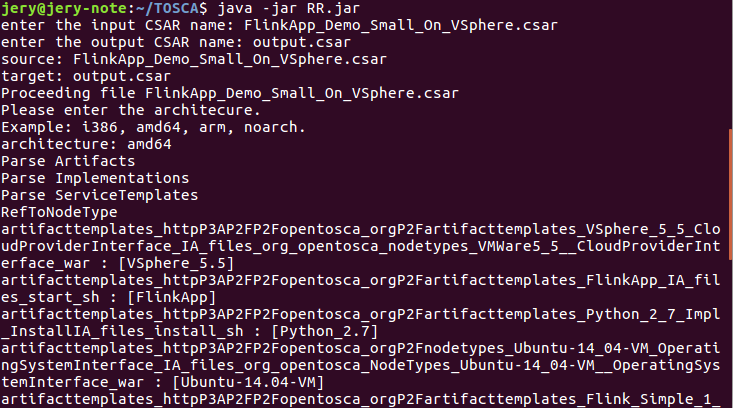
\includegraphics[width=0.7\textwidth]{Screenshot_processing}
	\caption{Processing by the framework.}
	\label{fig:process}
\end{figure}

\section{Displaying with Winery}\label{sec:checkwin}
Winery was installed to test the correctness of the output CSAR. 
 This is a tool for the development of TOSCA systems and is useful for checking the results. %\\
 The input CSAR's representation by Winery is displayed in Figure~\ref{fig:winery_source2}.
 Those external references will be resolved by the framework and exchanged by new nodes in output CSARs. 
 \begin{figure}[ht]   
 	\centering
 	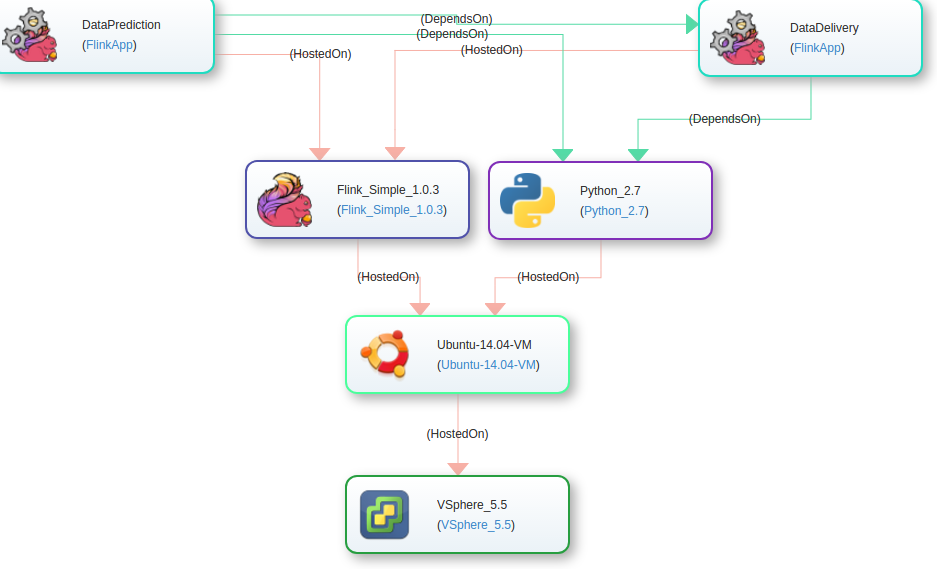
\includegraphics[width=0.7\textwidth]{Screenshot_winery_source2}
 	\caption{Source CSAR represented by $Winery$.}
 	\label{fig:winery_source2}
 \end{figure}
   
 \subsection*{Add to Winery}
 The output CSARs were added to Winery.
 Due to a significant increase in size of the default CSAR, this can be a fairly lengthy procedure.
 It was only six nodes in the input CSAR, but after the processing, the default CSAR contains more than 100 of nodes.
 Addition of a single node CSAR is faster process.
 The number of additional nodes coincides with the number of artifacts containing external references.
 During the addition to Winery, the CSAR's syntax is tested.
 In a case of errors, messages will be displayed.
 
 \subsection*{Display by Winery}
 The output CSARs were displayed by Winery.
Due to the high number of nodes, the processing of the default CSAR can take a long time. 
 At the time, the  internal references are validated.
 If something was defined not properly, these erroneous nodes or links between them will not be displayed.
The representation of the default CSAR is shown on Figure~\ref{fig:winery_output}, but only the part of the CSAR is visible.
 The structure seems very difficult to follow.
 To verify the topology some nodes was moved manually. 
 Figure~\ref{fig:winery_output2} displays the result. \\
 And figure~\ref{fig:winery_output_single} visualize the single node CSAR with manually moved nodes. 
 The correctness of dependencies was verified by checking several nodes with the $apt$-$cache$ $depends$ command.
 By opening the content of the new nodes, it was verified, that there are right artifacts.
 For example it was noted that python installing node from the single node CSAR contains more then 50 Deployment Artifacts and one Implementation Artifact which installs corresponding packages.
 \begin{figure}[ht]   
 	\centering
 	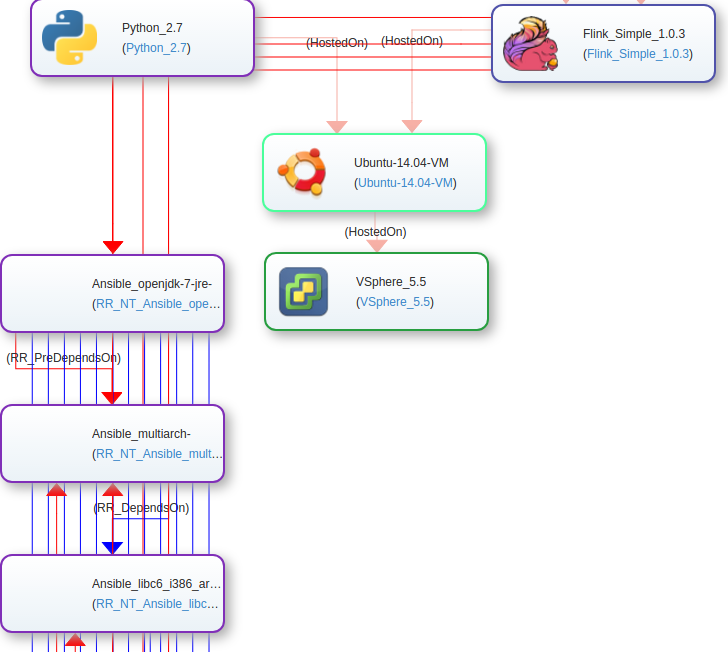
\includegraphics[width=0.7\textwidth]{Screenshot_winery_output}  
 	\caption{The CSAR processed in default mode and represented by Winery.}
 	\label{fig:winery_output}
 \end{figure}
 \begin{figure}[ht]   
 	\centering
 	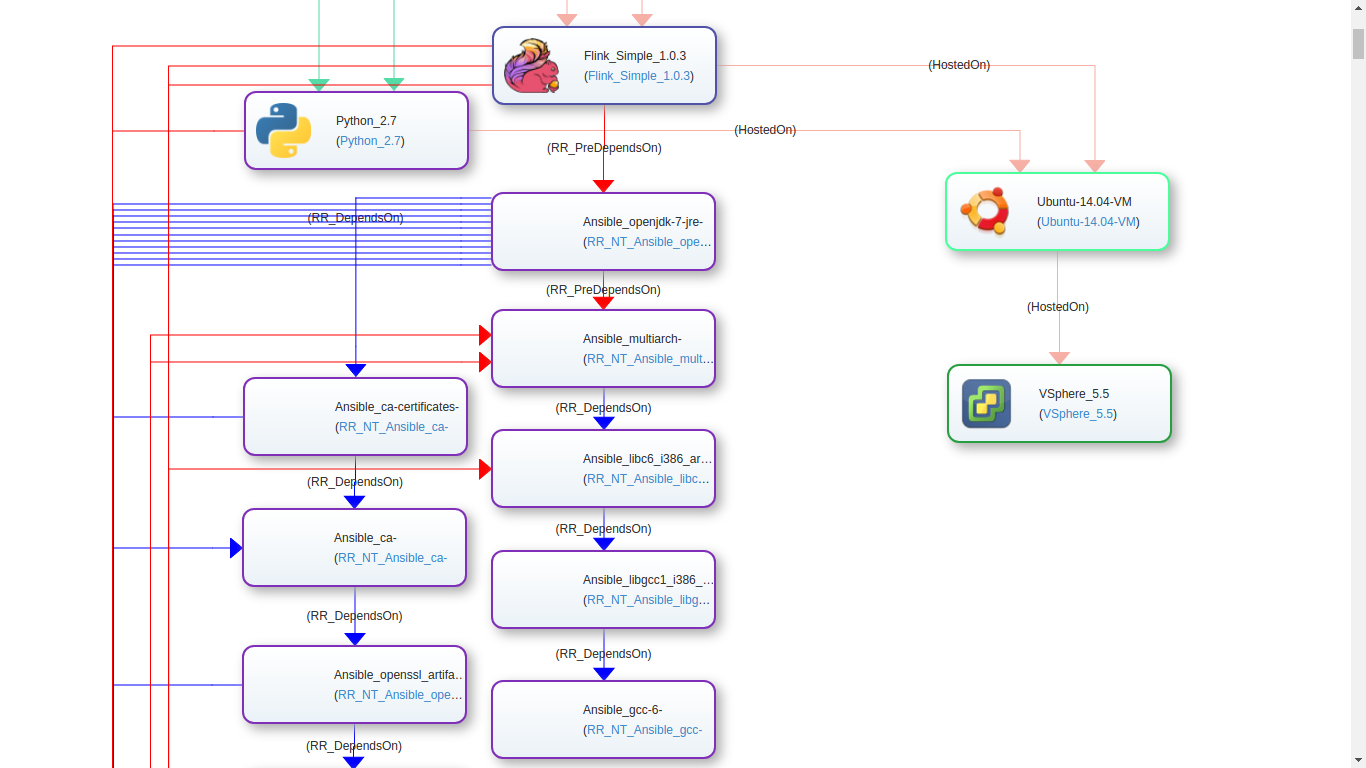
\includegraphics[width=0.7\textwidth]{Screenshot_winery_output2}
 	\caption{The default CSAR represented by Winery with some nodes moved manually.}
 	\label{fig:winery_output2}
 \end{figure}
\begin{figure}[ht]   
	\centering
	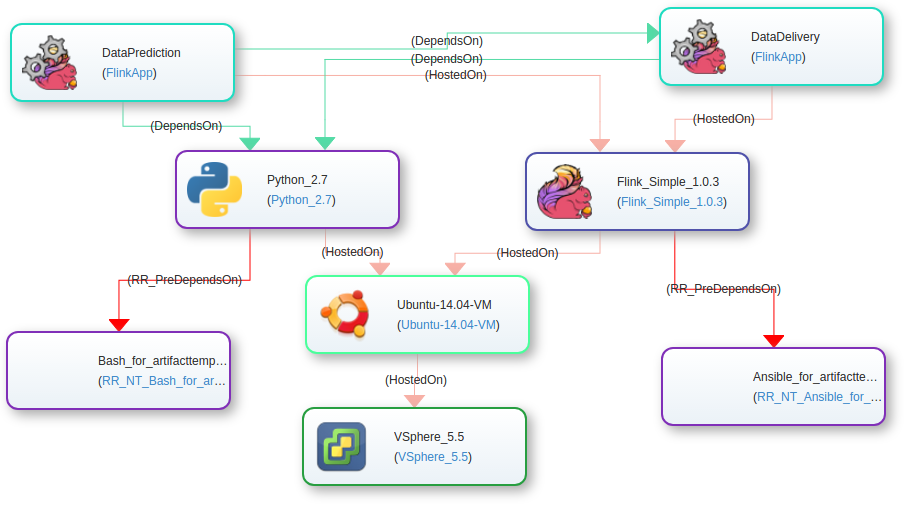
\includegraphics[width=0.7\textwidth]{Screenshot_winery_output_single}
	\caption{The representation of the CSAR processed in the single node mode.}
	\label{fig:winery_output_single}
\end{figure}
\section{Validate Artifacts}\label{sec:checkart}
It is necessary to check whether it is possible to install new packages using the generated artifacts.
At first Bash scripts will be tested, then ansible playbooks.

\subsection*{Validate Bash Scripts}
Since Bash is used in the Linux's command line, it will be pretty easy to check Bash installation scripts by starting them.
Of course that must be done with the necessary privileges.
An example of the $python2.7$ installation is presented in listing~\ref{lst:check_bash_script}. %\\
The process ended without any warnings or errors, which means that it was completed successfully.
This way any Bash installation script can be checked.
\begin{Listing}
	\caption{Check Bash installation script}
	\label{lst:check_bash_script}
	\begin{lstlisting}
	user@user:~$ sudo RR_python2_7-minimal.sh 
	(Reading database ... 286091 files and directories currently installed.)
	Preparing to unpack python2_7-minimal.deb ...
	Unpacking python2.7-minimal (2.7.12-1ubuntu0~16.04.1) over (2.7.12-1ubuntu0~16.04.1) ...
	Setting up python2.7-minimal (2.7.12-1ubuntu0~16.04.1) ...
	Processing triggers for man-db (2.7.5-1) ...
	\end{lstlisting}
\end{Listing}

\subsection*{Validate Ansible Playbooks}
To check an ansible playbook we need to extract the zip file containing the playbook manually. 
During the regular execution, this work will be done by a runtime environment.
The call of the ansible runtime which proceeds the playbook is a simple procedure too.
An example is provided in Figure~\ref{fig:ansible_output2}. %\\
$Ok$ signals that the installation was completed successfully.
\begin{figure}[ht]   
	\centering
	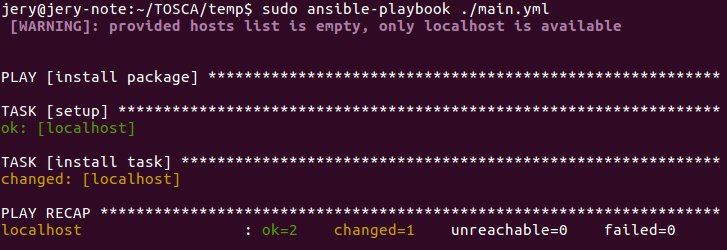
\includegraphics[width=0.7\textwidth]{Screenshot_ansible_output}
	\caption{An ansible playbook's execution process}
	\label{fig:ansible_output2}
\end{figure}